\documentclass[twocolumn]{article}
\usepackage{amsmath}
\usepackage{tabularx}
\usepackage{cite}
\usepackage{graphicx}
\title{excersice}
\date{}
\begin{document}
	\maketitle
		\section{Text}
	A distinct division of written or printed matter that begins on a new, usually indented line, consists of one or more sentences, and typically deals with a single thought or topic or quotes one speaker's continuous words. 
	\section{Symbols}
	this paragrah is taking about $\beta$ and it is so importantParagraphs are the building blocks of papers. Many students define paragraphs in terms of length: a paragraph is a group of at least five sentences, a paragraph is half a page long, etc \cite{pv}. In reality, though, the unity and coherence of ideas among sentences is what constitutes a paragraph. A paragraph is defined as “a group of sentences or a single sentence that forms a unit” (Lunsford and Connors 116). Length and appearance do not determine whether a section in a paper is a paragraph. For instance, in some styles of writing, particularly journalistic styles, a paragraph can be just one sentence long. Ultimately, a paragraph is a sentence or group of sentences that support one main idea. In this handout, we will refer to this as the “controlling idea,” because it controls what happens in the rest of the paragraph as shown in the table (\ref{tab:Drinks}).
\section{equation}
	\begin{equation*}
		x=cos(y)+\beta
\end{equation*}
\section{item}
	\begin{itemize}
		\item mohamed raffat
		\item ibrahim mohammed
\end{itemize}
\begin{enumerate}
		\item cat
		\item dog
\end{enumerate}
\section{advenced equation}
\begin{align*}
	(x+2)^3&=(x+2)(x+2)(x+2)\\
	&=(x+2)(x^2+4x+4)\\
	&=(x^3+6x^2+12x+8)
\end{align*}
	
\section{Tables}
\begin{table}[b]
	\centering
	\caption{Drinks}
	\label{tab:Drinks}
	\begin{tabular}{|c|c|c|}
		\hline
		item&qty&price\\
		\hline
		tea&3&30\\
		\hline %horizental line
		coffee&1&15\\
		\hline
	\end{tabular}
\end{table}

\section{citation}
\bibliographystyle{plain}	
\bibliography{red}
\section{figure}
\begin{figure}
	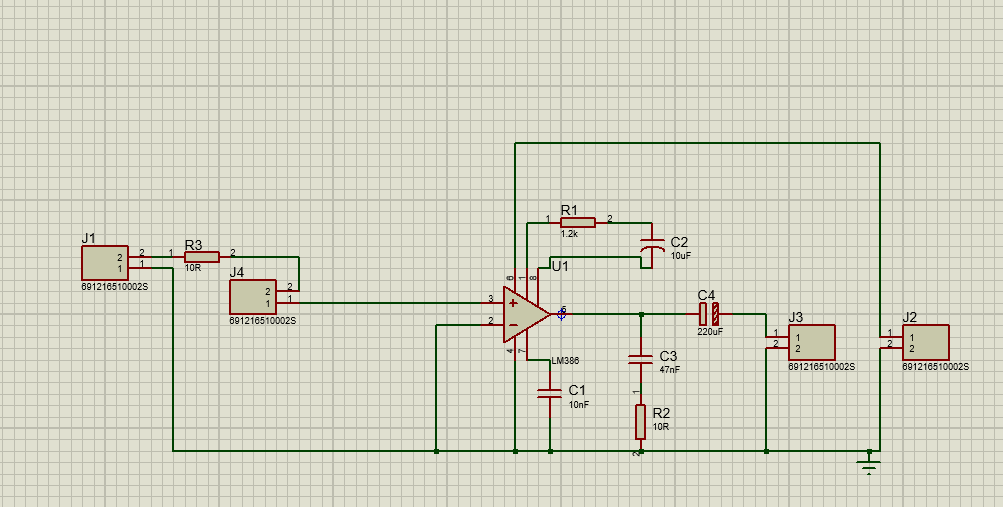
\includegraphics[width=0.9\columnwidth]{ampilifier}
	\caption{circuit}
\end{figure}
\begin{multline}
	\hat{y_{i}}=\sum_{j=1}^{N}a_{ij}x_{j}l_{j}/\rho_{j}
\end{multline}
\section{myeqitiom}
\begin{align}
E[a_{ij}x_{j}l_{j}] = a_{ij}x_{j}\cdot 0.5\\
E[\hat{y_{i}}] = \sum_{j=1}^{N}E[a_{ij}x_{j}l_{j}] = \sum_{j=1}^{N}0.5a_{ij}x_{j}\\
\sum_{j=1}^{N}0.5a_{ij}x_{j} = y_{i}\\
loss = \sum_{i=1}^{N}(y_{i} - \hat{y_{i}})^2
\end{align}
\end{document}
